\documentclass[a4paper,12pt]{scrartcl}
\usepackage[utf8]{inputenc}
\usepackage[ngerman]{babel}
\usepackage{amsmath,amssymb,amsthm}
\usepackage{graphicx}
\usepackage[onehalfspacing]{setspace}
\usepackage[colorlinks,
pdfpagelabels,
pdfstartview = FitH,
bookmarksopen = true,
bookmarksnumbered = true,
linkcolor = black,
plainpages = false,
hypertexnames = false,
citecolor = black] {hyperref}
\newtheorem{theorem}{Satz}[section]
\newtheorem{lemma}[theorem]{Lemma}
\newtheorem{bem}[theorem]{Bemerkung}
\newtheorem{defi}[theorem]{Definition}
\newcommand{\OR}[1]{{\mathcal{O}(\mathbb{R}^#1)}}
\begin{document}

\begin{titlepage}
\begin{center}

% Upper part of the page. The '~' is needed because \\
% only works if a paragraph has started.
% \includegraphics[width=0.15\textwidth]{./logo}~\\[1cm]

\textsc{\LARGE Universität Duisburg-Essen}\\[1.5cm]

\textsc{\Large Seminarvortrag}\\[0.5cm]

% Title
{ \huge \bfseries Endliche Drehgruppen im zwei- und dreidimensionalen Raum \\[0.4cm] }

% Author and supervisor
\begin{minipage}{0.4\textwidth}
\begin{flushleft} \large
\emph{Autor:}\\
Mike Barkmin
\end{flushleft}
\end{minipage}
\begin{minipage}{0.4\textwidth}
\begin{flushright} \large
\emph{Seminarleiter:} \\
Dr. Ingo Janiszczak
\end{flushright}
\end{minipage}

\vfill

% Bottom of the page
{\large \today}
%\setcounter{tocdepth}{1}
%\tableofcontents
\end{center}
\end{titlepage}
\newpage
\setcounter{tocdepth}{1}
\tableofcontents
\newpage
\section{Orthogonale Transformationen im zweidimensionalen Raum}
\begin{bem}
 Sei $T \in \mathcal{O}(\mathbb{R}^2)$, dann ist $T$ eindeutig über die Basisvektoren $e_1=(1,0)$ und $e_2=(0,1)$ definiert. Da $T \in \mathcal{O}(\mathbb{R}^2)$ und somit längen- und orthogonalitätserhaltend ist, existiert ein eindeutiges $\theta \in [0,2 \pi)$, sodass $Te_1=(\cos(\theta),\sin(\theta))$ und $Te_2=\pm(-\sin(\theta),\cos(\theta))$.

 Wenn $Te_2=(-\sin(\theta),\cos(\theta))$, dann wird $T$ durch die Matrix
 \begin{center}
  $A = \begin{pmatrix}
        \cos(\theta) && -\sin(\theta) \\
        \sin(\theta) && \cos(\theta)
       \end{pmatrix}$

 \end{center}
repräsentiert und $T$ ist eine Drehung um den Ursprung mit dem Winkel $\theta$. Außerdem gilt $\det T = \det A = \cos^2(\theta) + \sin^2(\theta) = 1$

Wenn $Te_2=(\sin(\theta),-\cos(\theta))$, dann wird $T$ durch die Matrix
 \begin{center}
  $A = \begin{pmatrix}
        \cos(\theta) && \sin(\theta) \\
        \sin(\theta) && -\cos(\theta)
       \end{pmatrix}$

 \end{center}
repräsentiert und $T$ ist eine Spiegelung. Außerdem gilt $\det T = \det A = -1$.
\end{bem}
\begin{theorem}
 Jede orthogonale Transformation im zweidimensionalen Raum ist entweder eine Spiegelung oder eine Drehung.
\end{theorem}

\newpage
\section{Endliche Gruppen im zweidimensionalen Raum}
\begin{theorem}
 Sei $\mathcal{G}$ eine endliche Untergruppe von $\OR{2}$, dann ist $\mathcal{G}$ entweder eine zyklische Gruppe $\mathcal{C}^n_2$ oder eine Diedergruppe $\mathcal{H}^n_2$ für $n \in \mathbb{N}$
\end{theorem}
\begin{proof}
 Wir nehmen an, dass $\mathcal{H} \leq \mathcal{G}$ durch die Menge aller Drehungen in $\mathcal{G}$ gebildet wird.
 
 Wir wollen zeigen, dass $\mathcal{H}$ zyklisch sein muss. Für $|\mathcal{H}|=1$ ist dieses bereits klar. Wenn $|\mathcal{H}| \neq 1$ wählen wir eine Drehung $R \in \mathcal{H}$, sodass $R \neq E_2$ und der Drehwinkel $\theta(R)$ minimal ist. Wenn wir jetzt eine weitere Drehung $T \in \mathcal{H}$ nehmen, dann können wir ein $m \in \mathbb{Z}$ finden, sodass \begin{align*}
        &m \theta(R)\leq\theta(T)<(m+1)\theta(R) \\
        \Leftrightarrow \ &0 \leq \theta(T)-m\theta(R)<\theta(R) \\
        \Leftrightarrow \ &0 \leq \theta(TR^{-m})<\theta(R)                                                                                                                                                                                                                                                                                                                                                           
\end{align*}
Da wir $\theta(R)$ minimal gewählt haben, gilt $\theta(TR^{-m})=0$. Also muss $TR^{-m}=E_2$ sein und es folgt $T=R^{m}$. Demnach ist $\mathcal{H}$ zyklisch mit $\mathcal{H}=<R>$ ($R$ ist Erzeuger von $\mathcal{H}$). Damit folgt auch, dass $\theta(R)=\frac{2}{n}\pi$, wenn $n=|\mathcal{H}|$. Wenn $\mathcal{G} = \mathcal{H}$ gilt, dann haben wir gezeigt, dass $\mathcal{G}$ zyklisch ist und wir bezeichnen $\mathcal{G}$ mit $\mathcal{C}^n_2$.

Als nächstes nehmen wir dann an, dass $\mathcal{G} \neq \mathcal{H}$ und wählen eine Spiegelung $S \in \mathcal{G}$. Nun wählen wir eine weitere beliebige Spiegelung $T \in \mathcal{G}$ mit $T \neq S$, dann gilt $\det(ST)=\det(S)\det(T)=1$. Deshalb gilt $ST \in \mathcal{H}$ und es handelt sich bei $ST$ um eine Drehung. Dann gilt $T \in S\mathcal{H}$, da $S^{-1}=S$. So gilt, dass $\mathcal{H}$ eine Untergruppe von $\mathcal{G}$ mit Index $2$ ist und $\mathcal{H}=<R>$. Dann gilt $\mathcal{G}=<R,S>$ $=\{E_2,R,\dots \ ,R^{n-1},S,SR,\dots ,SR^{n-1}$\} und $|\mathcal{G}|=2n$. Da $RS$ eine Spiegelung ist, gilt $(RS)^2=E_2$ und $RS=SR^{-1}=SR^{n-1}$, damit sind alle Verknüpfungen in $\mathcal{G}$ festgelegt. Die Gruppe $\mathcal{G}$ bezeichnen wir mit $\mathcal{H}^n_2=<S,R>$ (Die Diedergruppe von Ordnung 2n).                                                                                                                                                                                                                                                                                                                                                           
\end{proof}


\newpage
\section{Orthogonale Transformationen im dreidimensionalen Raum}
\begin{theorem}
 Angenommen $T$ ist eine Drehung in $\OR{3}$, dann ist $T$ eine Drehung um eine fixierte Achse, sodass $T$ einen Eigenvektor $x$ zum Eigenwert $1$ besitzt und die Einschränkung von $T$ auf die Ebene $\mathcal{P}=x^{\perp}$ eine Drehung im zweidimensionalen Raum ist.
\end{theorem}
\begin{proof}
 Angenommen $T$ ist eine Drehung in $\OR(3)$ und $\lambda_1,\lambda_2,\lambda_3$ sind Eigenwerte von $T$. Sei $\lambda_1 \in \mathbb{R}$, dann können $\lambda_2$ und $\lambda_3$ nur folgende Werte annehmen, da $\det(T)=\lambda_1\lambda_2\lambda_3=1$.
 \begin{align}
  \lambda_1=1, \lambda_2=\lambda_3=\pm1 \\
  \lambda_1=1, \lambda_2=\overline{\lambda_3}\notin \mathbb{R}
 \end{align}
Für uns ist aber nur der Eigenwert $1$ interessant, dieser ist aber in beiden Fällen vorhanden.

Wir wählen einen Eigenvektor $x$ zum Eigenwert $1$ und bemerken, dass $x=T^{-1}Tx=T^{-1}x$ gilt. Deshalb gilt auch $0=(x^{\perp},x)=(x^{\perp},T^{-1}x)=(Tx^{\perp},x)$ und $\mathcal{P}=x^{\perp}$ ist invariant unter $T$. Betrachten wir nun die Determinate der Einschränkung $T|\mathcal{P}$, dann gilt $\det(T|\mathcal{P})=1$. Demnach ist $T|\mathcal{P}$ eine Drehung der Ebene $\mathcal{P}$
\end{proof}
\begin{bem}
 Wenn $S$ eine Spiegelung an der Ebene $\mathcal{P}$ in $\OR(3)$ ist, dann gilt $Sx=x \ \forall x \in \mathcal{P}$ und $Sy=-y \ \forall y \in \mathcal{P}^{\perp}$. Wir können nun einen Einheitsvektor $r \in \mathcal{P}^{\perp}$ so wählen, dass $Sx=x-2(x,r)r \ \forall x\in \mathbb{R}^3$ gilt. Wenn wir nun eine Basis $\{r,x_2,x_3\}$ von $\mathcal{P}$ wählen, sodass die Transformationsmatirx unter dieser Basis von $S$ durch 
 \begin{center}
  $A= \begin{pmatrix}
        -1 && 0 && 0 \\
        0 && 1 && 0 \\
        0 && 0 && 1 
       \end{pmatrix}$
 \end{center}
repräsentiert wird. Es gilt außerdem $S^2 = E_3$.
\end{bem}
\begin{theorem}
 Sei $T\in\OR{3}$ mit $det T = -1$. Dann ist $T$ eine Drehspiegelung mit Spiegelebene $\mathcal{P}$ und Drehachse $\mathcal{P}^{\perp}$.
\end{theorem}
\begin{proof}
 Angenommen $T$ ist eine Spiegelung in $\OR(3)$ und $\lambda_1,\lambda_2,\lambda_3$ sind Eigenwerte von $T$. Sei $\lambda_1 \in \mathbb{R}$, dann können $\lambda_2$ und $\lambda_3$ nur folgende Werte annehmen, da $\det(T)=\lambda_1\lambda_2\lambda_3=-1$.
 \setcounter{equation}{0}
 \begin{align}
  \lambda_1=-1, \lambda_2=\lambda_3=\pm1 \\
  \lambda_1=-1, \lambda_2=\overline{\lambda_3}\notin \mathbb{R}
 \end{align}
 Wir wählen einen Eigenvektor $x$ zum Eigenwert $-1$ und wählen $\mathcal{P}=x^{\perp}$. Betrachten wir nur die Determinate der Einschränkung $T|\mathcal{P}$, also $det(T|\mathcal{P})=\lambda_2\lambda_3=1$, dann lässt sich erkennen, dass $T|\mathcal{P}$ eine Drehung der Ebene $\mathcal{P}$ sein muss. Wir wählen nun eine Basis $\{x_1,x_2\}$ von $\mathcal{P}$, sodass die Transformationsmatirx von $T$ unter der Basis $\{x_1,x_2,x_3\}$ durch \begin{align*}
  A&=
\begin{pmatrix}
        -1 && 0 && 0 \\
        0 && \cos(\theta) && -\sin(\theta) \\
        0 && \sin(\theta) && \cos(\theta)
       \end{pmatrix} \\ &=
       \begin{pmatrix}
        1 && 0 && 0 \\
        0 && \cos(\theta) && -\sin(\theta) \\
        0 && \sin(\theta) && \cos(\theta)
       \end{pmatrix} 
       \begin{pmatrix}
        -1 && 0 && 0 \\
        0 && 1 && 0 \\
        0 && 0 && 1
       \end{pmatrix}
 \end{align*}
repräsentiert wird.
\end{proof}




\newpage
\section{Endliche Drehgruppen im dreidimensionalen Raum}
\begin{bem}
 Sei $W$ ein Untervektorraum mit $\dim W = 2$ im Vektorraum V mit $\dim V = 3$. Wenn $R$ eine Drehung in $\mathcal{O}(W)$ ist, dann kann $R$ zu einer Drehung in $\mathcal{O}(V)$ erweitert werden. Dazu wählen wir eine Basis $\{x_1,x_2,x_3\}$ von $V$ mit $x_1 \in W^{\perp}$ und $x_2,x_3 \in W$, sodass die Matrix $R$ von \begin{center}
                                                                                                                                                                                                                                                                                                                                 $A=\begin{pmatrix}                                                                                                                                                                                                                                                                                                                                     
   1 && 0 && 0 \\
   0 && \cos(\theta) && -\sin(\theta) \\
   0 && \sin(\theta) && \cos(\theta)
   \end{pmatrix}
$                                                                                                                                                                                                                                                                                                                         \end{center}
repräsentiert wird.
\end{bem}
\begin{bem}
 Wenn wir jede Transformation $T$ aus einer Diederuntergruppe $\mathcal{H}^n_2$ zu einer Drehung in $\mathcal{O}(V)$ erweitern, dann erhalten wir eine Menge von Drehungen die eine Untergruppe von $\mathcal{O}(V)$ bilden und diese Untergruppe ist isomorph zu $\mathcal{H}^n_2$. Wir bezeichnen sie als Diedergruppe $\mathcal{H}^n_3$.
\end{bem}
\subsection{Platonische Körper}
 Da endliche Untergruppen von $\OR{2}$ Symmetriegruppen von regelmäßigen Polygonen sind, ist es naheliegend, dass wir uns nun mit regelmäßigen Polyedern beschäftigen. Es gibt genau 5 regelmäßige Polyeder, die sogenannten platonischen Körper. 
 
 Wenn wir ein regelmäßiges Polyeder am Ursprung des $\mathbb{R}^3$ ausrichten, dann sind die Drehungen die das Polyeder wieder in sich überführen eine endliche Untergruppe von $\OR(3)$. Auf diese Art entstehen drei unterschiedliche endliche Gruppen von Drehungen. Denn der Würfel besitzt die gleiche Menge von Drehungen wie das Oktaeder und das Ikosaeder besitzt die gleiche Menge von Drehungen wie das Dodekaeder. Die folgende Illustration verdeutlicht warum dies der Fall ist.
 \\  \\
 \begin{center}
 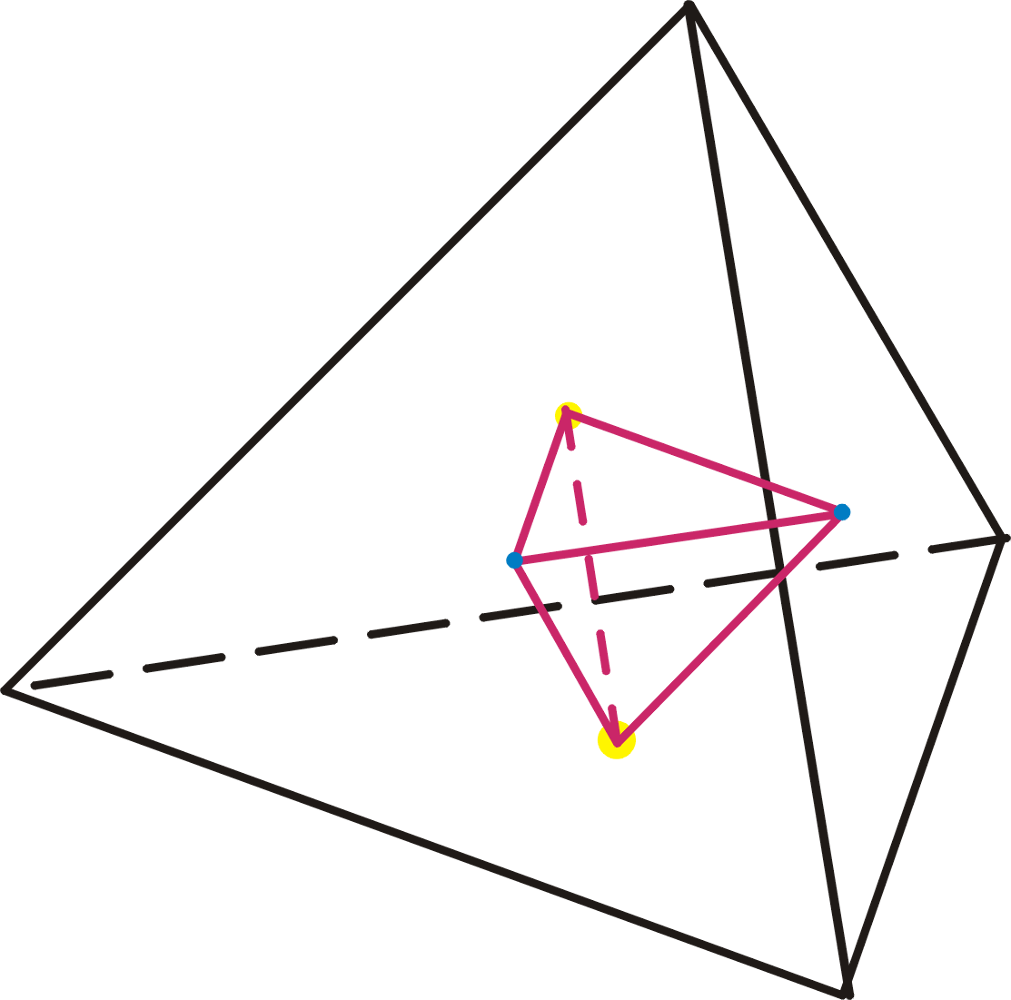
\includegraphics[height=110px]{./Grafiken/Duality_Tetra-Tetra.png} \ \
 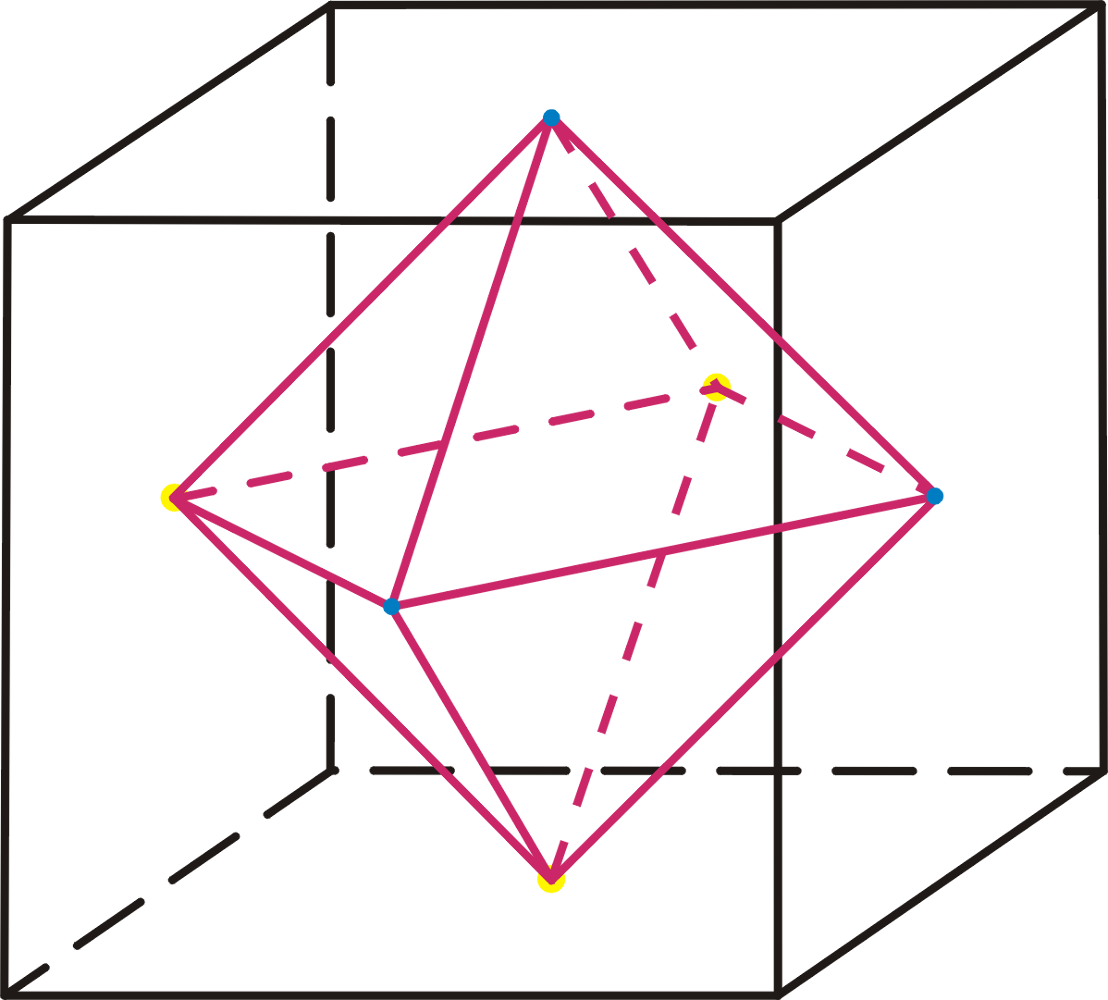
\includegraphics[height=110px]{./Grafiken/Duality_Hexa-Okta.png} \ \
 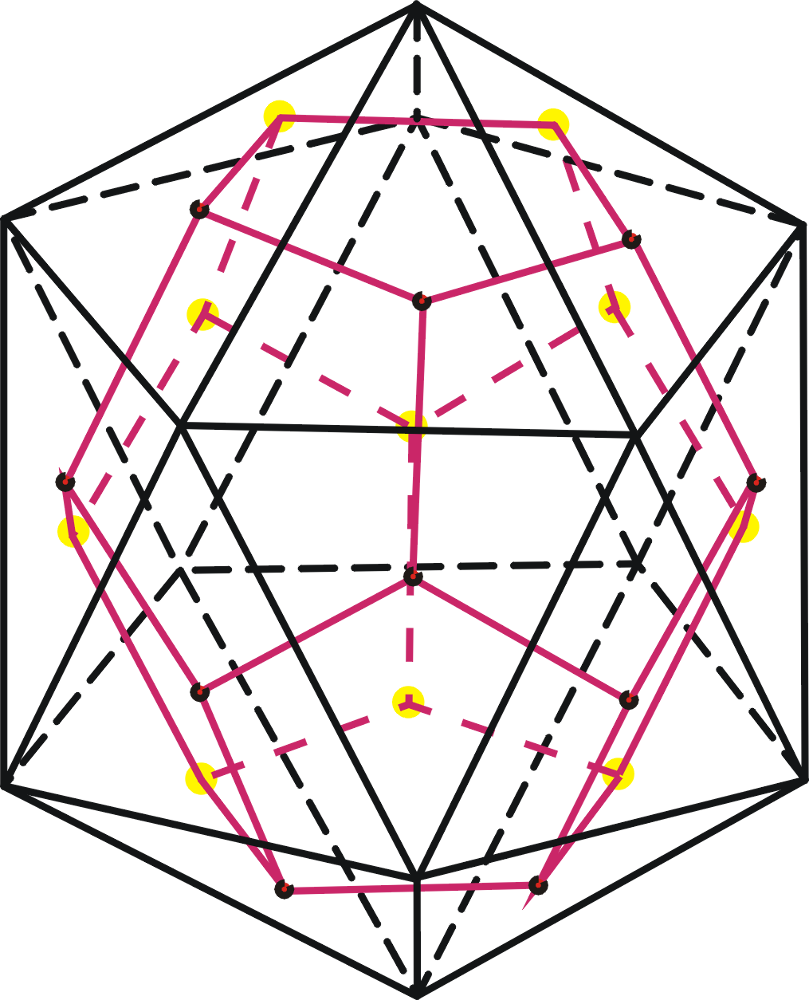
\includegraphics[height=110px]{./Grafiken/Duality_Iko-Dodek.png}
 \end{center}
 \newpage
Aus der Skizze lassen sich auch die Drehungen, die die Körper in sich überführen, leicht ablesen. Wir den nächsten Abschnitt nehmen wir an, dass die Körper immer mit ihrem Schwerpunkt im Ursprung vom $\mathbb{R}^3$ liegen.

Zunächst betrachten wir die Untergruppe $\mathcal{T}$ der Drehungen von $\OR{3}$ des Tetraeders. Diese besitzt
\begin{itemize}
  \item die Identität
  \item 8 Drehungen, um die Drehachsen zwischen einem Eckpunkte und dem Mittelpunkt de rgegenüberliegenden Seite mit Drehwinkel $\frac{2}{3}\pi,\frac{4}{3}\pi$
  \item 3 Drehungen, um die Drehachsen zwischen den Mittelpunkten zweier gegenüberliegender Kanten mit Drehwinkel $\pi$
\end{itemize}
Es gilt somit $|\mathcal{T}|=4 \cdot 2 + 3 \cdot 1 +1 = 12$

Als nächstes betrachen wir die Untergruppe $\mathcal{W}$ der Drehungen von $\OR{3}$ des Würfels. Diese besitzt
\begin{itemize} 
  \item die Identität
  \item 9 Drehungen, um die Drehachsen zwischen den Mittelpunkten zweier gegenüberliegender Seiten mit Drehwinkel $\frac{1}{2}\pi,\pi,\frac{3}{2}\pi$
  \item 8 Drehungen, um die Drehachsen zwischen zwei gegenüberliegenden Eckpunkten mit Drehwinkel $\frac{2}{3}\pi,\frac{4}{3}\pi$
  \item 6 Drehungen, um die Drehachsen zwischen den Mittelpunkten zweier gegenüberliegenden Kanten mit Drehwinkel $\pi$
\end{itemize}
Es gilt somit $|\mathcal{W}|=6 \cdot 1 + 4 \cdot 2 + 3 \cdot 3 +1 = 24$

Zuletzt betrachen wir die Untergruppe $\mathcal{I}$ der Drehungen von $\OR{3}$ des Ikosaeders. Diese besitzt
\begin{itemize} 
  \item die Identität
  \item 24 Drehungen, um die Drehachsen zwischen den Mittelpunkten zweier gegenüberliegender Eckpunkte mit Drehwinkel $\frac{2}{5}\pi,\frac{4}{5}\pi,\frac{6}{5}\pi,\frac{8}{5}\pi$
  \item 20 Drehungen, um die Drehachsen zwischen den Mittelpunkten zweier gegenüberliegender Seiten mit Drehwinkel $\frac{2}{3}\pi,\frac{4}{3}\pi$
  \item 15 Drehungen, um die Drehachsen zwischen den Mittelpunkten zweier gegenüberliegender Kanten mit Drehwinkel $\pi$
\end{itemize}
Es gilt somit $|\mathcal{I}|=15 \cdot 1 + 10 \cdot 2 + 6 \cdot 4 +1 = 60$
\begin{defi}
 Sei $E_3 \neq T \in \OR{3}$ eine Drehung, dann hat $T$ genau zwei Fixpunkte auf der Einheitskugel, nämlich die Schnittpunkte der Einheitskugel mit der Drehachse. Diese Punkte nennen wir die Pole der Drehung.
\end{defi}
\begin{lemma}
 Sei $\mathcal{G} \leq \OR{3}$, dann ist $\mathcal{G}$ eine Permutationsgruppe auf der Menge $\mathcal{P}$ ihrer Pole.
\end{lemma}
\begin{proof}
 Wenn $x \in \mathcal{P}$ ist, dann ist $x$ ein Pol einer Drehung $T \in \mathcal{G}$ mit $T \neq E_3$. Für jede Drehung $R \in \mathcal{G}$ wissen wir $Rx=RTx=(RTR^{-1})Rx$. Also ist $Rx$ ein Pol der Drehung $RTR^{-1}$ zbd $Rx \in \mathcal{P}$.
\end{proof}
\begin{bem}
 Wenn wir uns die Bahen, Ordnung der Stabilisatoren und die Anzahl der Pole einer Symmetriegruppe $G$ mit Polmenge $P$ anschauen, dann ergeben sich folgende charakteristische Werte. \\
 {%
\newcommand{\mc}[3]{\multicolumn{#1}{#2}{#3}}
\begin{center}
\begin{tabular}{l|ccccll}
$\mathcal{G}$ & $|\mathcal{G}|$ & $|\mathcal{P}|$ & Anzahl Bahnen & \mc{3}{c}{Ordnung der Stabilisatoren}\\
\hline
$\mathcal{C}^n_2$ & n & 2 & 2 & 2 & \mc{1}{c}{2} & \mc{1}{c}{n}\\
$\mathcal{H}^n_3$ & 2n & 2n + 2 & 3 & 2 & \mc{1}{c}{3} & \mc{1}{c}{3}\\
$\mathcal{T}$ & 12 & 14 & 3 & 2 & \mc{1}{c}{3} & \mc{1}{c}{4}\\
$\mathcal{W}$ & 24 & 26 & 3 & 2 & \mc{1}{c}{3} & \mc{1}{c}{4}\\
$\mathcal{I}$ & 60 & 62 & 3 & 2 & \mc{1}{c}{3} & \mc{1}{c}{5}
 \end{tabular}
 \end{center}
}%
Damit haben wir eine komplette Aufzählung aller endlichen Untergruppen von Drehungen in $\OR{3}$ gefunden.
\end{bem}
\begin{proof}
 ?????
\end{proof}





\newpage
\section{Endliche Gruppen im dreidimensionalen Raum} 
Nachdem wir die endlichen Drehgruppen im dreidimensionalen Raum klassifiziert haben, möchten wir nun die endlichen Gruppen klassifizieren. Wir schauen uns zunächst die Gruppe $\mathcal{W}^*$ an. Diese soll alle orthogonalen Abbildungen umfassen, welche den Würfel wieder auf sich selber abbilden. Natürlich ist leicht zu sehen, dass $\mathcal{W}$ kleiner ist als $\mathcal{W}^*$. Aber wir können bemerken, dass für $T \in \mathcal{W}^*\backslash\mathcal{W}$ \ $-T = -1 \cdot T \in \mathcal{W}$ gilt. Daher gilt $\mathcal{W}^*=\mathcal{W}\cup(-1)\mathcal{W}$ und wir können ohne Berücksichtigung der Dimension folgendes Lemma aufstellen.
\begin{lemma}
 Wenn $\mathcal{G}\leq\mathcal{O}(V)$ und $\mathcal{H}$ eine Untergruppe aus Drehungen von $\mathcal{G}$ ist, dann gilt entweder $\mathcal{H}=\mathcal{G}$ oder $[\mathcal{G}:\mathcal{H}]=2$. Insbesonder ist $\mathcal{H}$ eine Untergruppe von $\mathcal{G}$ 
\end{lemma}
\begin{proof}
 Angenommen $T\in\mathcal{G}\backslash\mathcal{H}$, dann können wir ein beliebiges $S\in\mathcal{G}\backslash\mathcal{H}$ finden, sodass $\det(T^{-1}S)=(-1)^2=1$ und $T^{-1}S\in\mathcal{H}$ gilt. Folglich ist dann $\mathcal{G}=\mathcal{H}\cup T \mathcal{H}$ und $[\mathcal{G}:\mathcal{H}]=2$
\end{proof}
\begin{theorem}
 Sei $\mathcal{G}\leq\OR{3}$, dann ist $\mathcal{G}$ isomorph zu einer der folgenden Klassen:
 \begin{itemize}
  \item $\mathcal{C}^n_3,n\geq1;\mathcal{H}^n_3,n\geq2;\mathcal{T};\mathcal{W};\mathcal{I}$
  \item $(\mathcal{C}^n_3)^*,n\geq1;(\mathcal{H}^n_3)^*,n\geq 2;\mathcal{T}^*;\mathcal{W}^*;\mathcal{I}^*$
  \item $\mathcal{C}^2n_3]\mathcal{C}^n_3,n\geq1;\mathcal{H}^n_3]\mathcal{C}^n_3,n\geq 2;\mathcal{H}^2n_3,n]\mathcal{H}^n_3,\geq2;\mathcal{W}]\mathcal{T}$
\end{itemize}
Hinweis: $\mathcal{R}^*:=\mathcal{R}\cup -\mathcal{R}$ und $\mathcal{R}]\mathcal{P}:=\mathcal{P}\cup \{-U|U\in \mathcal{R} \backslash \mathcal{P} \}$
\end{theorem}

\end{document}